\subsection{Overall structure of the work plan}

Our work plan is divided into seven scientific work packages.
The first group of work packages is dedicated to the networking
activities that are needed to gather the proofs today located in
different libraries.

\begin{longtable}{|p{0.05\textwidth}|p{0.2\textwidth}|p{0.65\textwidth}|}
\hline
\rowcolor{color2}\multicolumn{3}{|l|}{\bf Networking activities:}\\
\hline
WP1
&
Integration
&
Instrument the systems for which we already know how to encode the
proofs in Dedukti, and make available these proofs in Logipedia.
\\
\hline
WP2
&
Automatic theorem proving
& 
Develop automatic theorem provers to populate,
help, and benefit from Logipedia.
\\
\hline
WP3
&
Large libraries
&
Export large dedicated libraries in curated form 
to Logipedia for end-user applications.
\\
\hline
\end{longtable}

The second is dedicated to making these proofs accessible, beyond
trans-national and virtual access.

\begin{longtable}{|p{0.05\textwidth}|p{0.2\textwidth}|p{0.65\textwidth}|}
\hline
\rowcolor{color2}\multicolumn{3}{|l|}{\bf Trans-national and virtual access:}\\
\hline
WP4
&
Access
&
Define and build the Logipedia hardware and software infrastructure in
which the proofs will be integrated.
\\
\hline
WP5
&
Structure of the encyclopedia
&
Provide infrastructure for the structured ontological representation
of libraries and use it to enrich the information about formal
libraries in Logipedia.
\\
\hline
\end{longtable}

The third is dedicated to joint research activities that prepare
the future of Logipedia.

\begin{longtable}{|p{0.05\textwidth}|p{0.2\textwidth}|p{0.65\textwidth}|}
\hline
\rowcolor{color2}\multicolumn{3}{|l|}{\bf Joint research activities:}\\
\hline
WP6
&
Theories
&
Bringing proof systems implementing a theory 
that has not yet been expressed in Dedukti to LIL 2 or better.
\\
\hline
WP7
&
Proof engineering
&
Investigate methods for detecting concept alignments and apply
them to build a library of alignments present across the Logipedia database.
\\
\hline
\end{longtable}

Together with these seven scientific work packages, 
two more work packages are dedicated to dissemination, communication and
exploitation and to management.

\begin{longtable}{|p{0.05\textwidth}|p{0.2\textwidth}|p{0.65\textwidth}|}
\hline
\rowcolor{color2}\multicolumn{3}{|l|}{\bf Dissemination, communication, exploitation, and management:}\\
\hline
WP8
&
Dissemination, communication, and exploitation
&
Expand the use of Logipedia in research, industry, education, and publishing.
\\
\hline
WP9
&
Management
&
Coordinate this large community, in a benevolent atmosphere, for optimal
efficiency.
\\
\hline
\end{longtable}

These work packages are diverse in the number of tasks and
partners. Some of them are large, while others are smaller. This
reflects the diversity of their natures and goals. The work package
``access'' for instance has a very definite and critical goal, it must
have a small number of partners and be focused on its goal. In
contrast, the work package ``theories'' requires experts in many
different systems.  It therefore has a larger number of partners.

\wpfigstyle{\scriptsize\setlength{\tabcolsep}{2pt}}
\wpfig%[type]%pages,type,start,end]

%%%%%%%%%%%%%%%%%%%%%%%%%%%%%%%%%%%%%%%%%%%%%%%%%%%%%%%%%%%%%%%%%%%%%%%%%%%%%%
\subsection{Timing of the different work packages and their components}

{\color{red} Gantt chart}

%\ganttchart[draft,xscale=.32] 

\subsection{Detailed work description}

\begin{center}
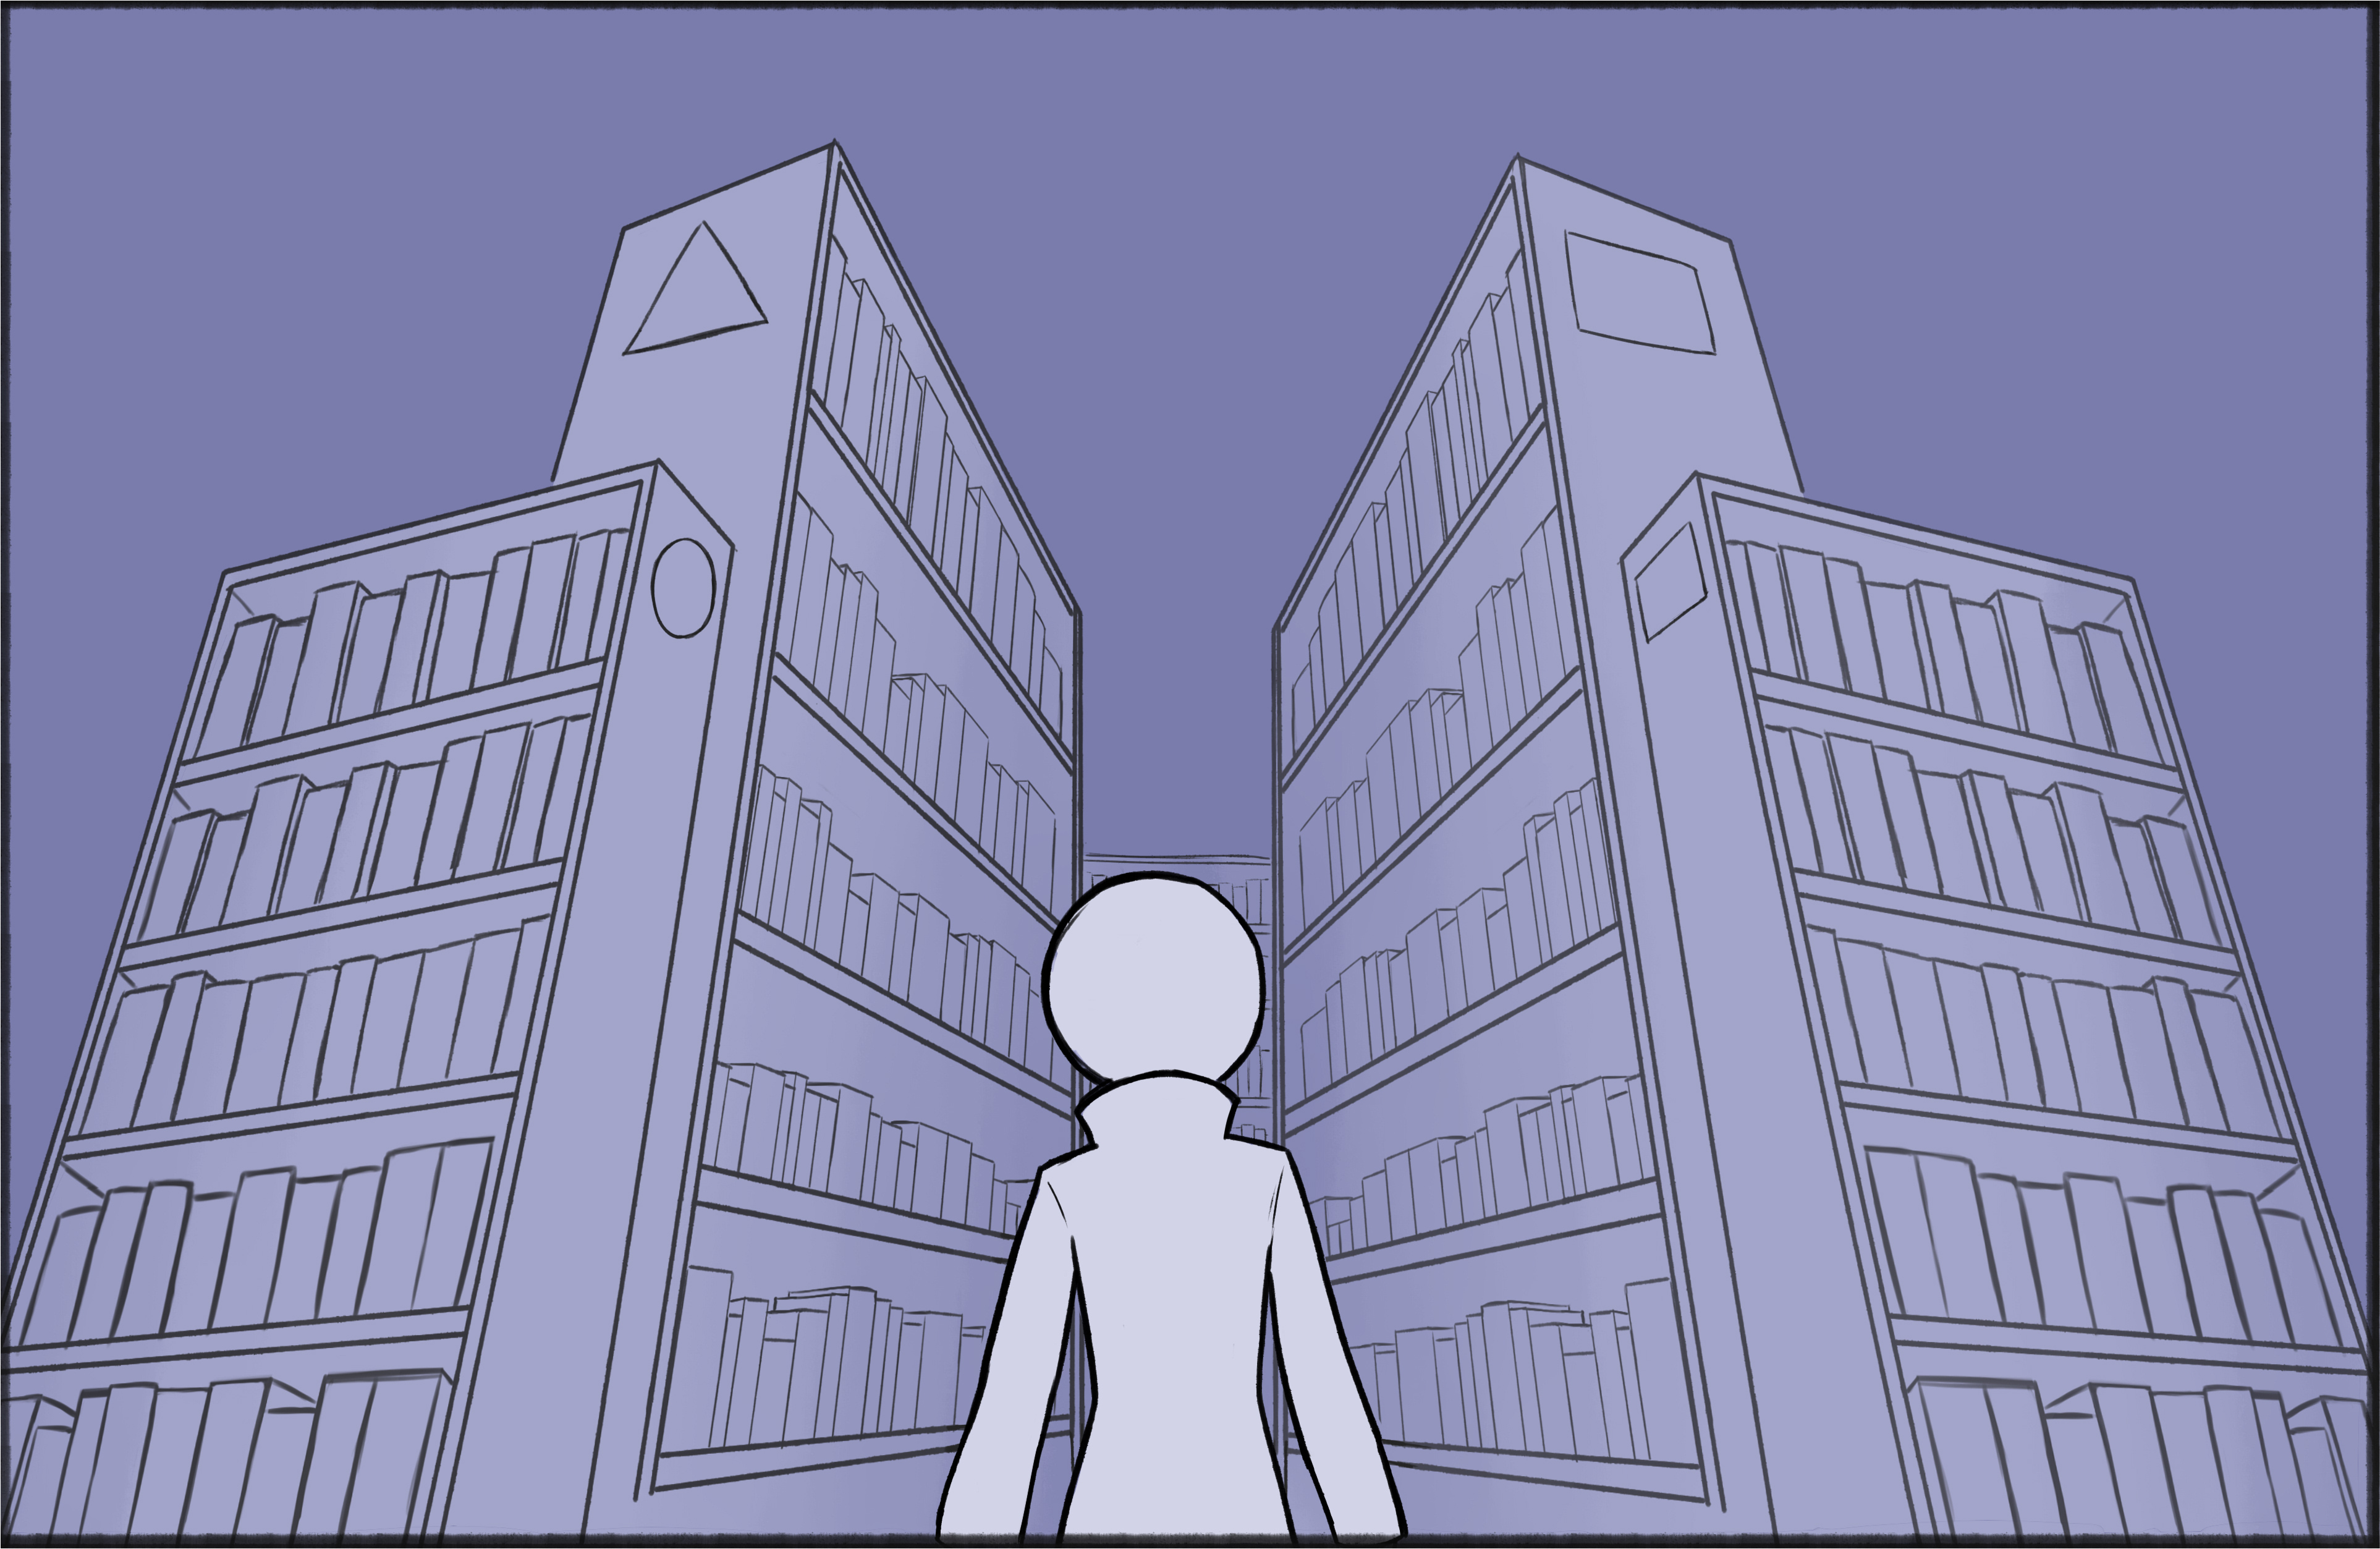
\includegraphics[width=7cm]{Illustration4_Color.jpg}
\end{center}

\begin{workplan}

% the template says: "indicate in the work package title the type of activity"

  \newcommand\na{(Networking activity)}
  \newcommand\tnva{(Trans-national and virtual access)}
  \newcommand\jra{(Joint research activity)}
  \newcommand\titlewp[3]{\bigskip\noindent\colorbox{color3}{\begin{minipage}\textwidth\bf Work Package #1: #2\end{minipage}}\input{workpackages/#3}}

\titlewp{1}{Integration \na}{instrumentation}

\titlewp{2}{Automatic theorem provers \na}{atpetc}

\titlewp{3}{Large libraries \na}{libraries}

\titlewp{4}{Accesses to the encyclopedia \tnva}{access}

\titlewp{5}{Structure of the encyclopedia \tnva}{structuring}

\titlewp{6}{Theories \jra}{theories}

\titlewp{7}{Proof engineering \jra}{alignment}

\titlewp{8}{Dissemination, communication and exploitation}{dissemination}

\titlewp{9}{Management}{management}

\end{workplan}

\subsubsection*{List of all deliverables}\label{sec:deliverables}

Here is an overview of the deliverables 
of the work packages. 

%In the table below, \emph{integrating work deliverables} (see top of
%section~\ref{sec:wplist}) are printed in boldface to mark them. They integrate
%contributions from multiple work packages.

{\footnotesize\inputdelivs{8cm}}

%%% Local Variables: 
%%% mode: latex
%%% TeX-master: "propB"
%%% End: 


%%%%%%%%%%%%%%%%%%%%%%%%%%%%%%%%%%%%%%%%%%%%%%%%%%%%%%%%%%%%%%%%%%%%%%%%%%%%%%
\subsection{Relation between the components}

{\color{red} Pert chart}
